\documentclass[border=5pt]{standalone}
\usepackage{tikz}
\usepackage{pgfplots}
\pgfplotsset{compat=1.18}
\usepackage{amsmath}
\tikzset{elegant/.style={smooth,thick,samples=50}}

\begin{document}
    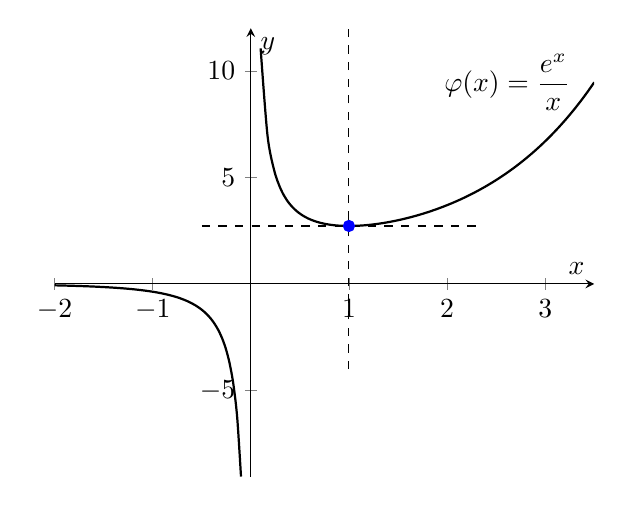
\begin{tikzpicture}
        \begin{axis}[
            axis x line = middle,
            axis y line = middle,
            ylabel = $y$,
            xlabel = $x$
        ]
        \addplot[elegant,domain=-2:-0.1]{exp(x)/x};
        \addplot[elegant,domain=0.1:3.5]{exp(x)/x} node [left=5pt] {$\varphi(x)=\dfrac{e^x}{x}$};
        \addplot[dashed] coordinates {(1,-4) (1,12)};
        \addplot[dashed] coordinates {(-0.5,e) (2.3,e)};
        \addplot[blue,mark=*] coordinates {(1,e)};
        \end{axis}
    \end{tikzpicture}
\end{document}